\chapter{Исследовательская часть}
В текущем разделе будут представлены примеры работы разработанного программного обеспечения, постановка эксперимента и сравнительный анализ реализованных алгоритмов.

\section{Пример работы программного обеспечения}

На рисунке \ref{fig:prog_exmpl} представлен результат работы программы при выбранном режиме построения --- с распараллеливанием, длине отрезка --- 300, количестве потоков --- 8. В результате выполнения программы на экране (канвас) появился спектр отрезков длины 300.

\begin{figure}[h!]
	
	\centering{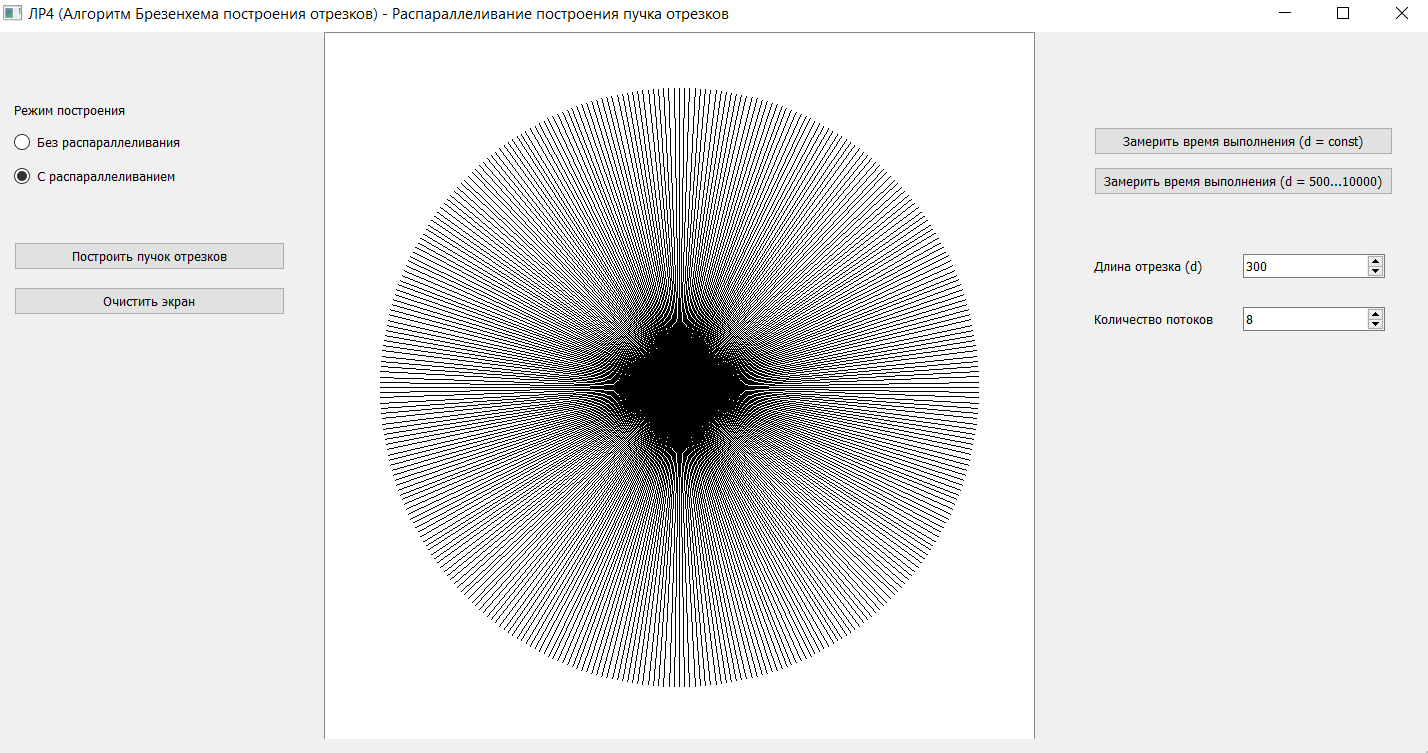
\includegraphics[scale=0.55]{inc/prog_exmpl.PNG}}
	
	\caption{Пример работы программы}
	
	\label{fig:prog_exmpl}
	
\end{figure}

\section{Технические характеристики}

Технические характеристики устройства, на котором выполнись замеры времени:

\begin{itemize}
	\item операционная система: Windows 10~\cite{windows10};
	\item оперативная память: 16 Гб;
	\item процессор: Intel® Core™ i5 10300H 2.5 ГГц;
	\item 4 физических ядра, 4 логических ядра.
\end{itemize}

Во время замеров времени выполнения реализаций алгоритмов ноутбук был включен в сеть питания и нагружен только встроенными приложениями окружения и системой тестирования.

\section{Время выполнения реализаций алгоритмов построения спектра отрезков}
Для замера времени выполнения реализованных алгоритмов использовалась функция \textit{system\_clock::now(...)} из библиотеки $chrono$. Данная функция возвращает время в наносекундах.

Использовать эту функцию необходимо дважды, затем из конечного времени нужно вычесть начальное, чтобы получить результат.

Замеры времени проводились для разной длины отрезка в спектре (от 1000 до 10000 с шагом 1000) и для разного количества потоков (1, 2, 4, 8, 16, 32), в качестве результата бралось среднее время из 500 итераций и переводилось из наносекунд в секунды посредством деления на $10^9$.

Результаты замеров времени работы реализаций алгоритмов приведены в таблицах \ref{tbl:time_mes_par}, \ref{tbl:time_mes_difdiam}.
\\
\\
\\
\\
\\
\\
\begin{table}[h]
    \begin{center}
        \caption{Результаты замеров времени (разное количество потоков, длина отрезка в спектре --- 500)}
        \label{tbl:time_mes_par}
        \begin{tabular}{|c|c|}
            \hline
            Количество потоков & Время выполнения (с) \\
            \hline
            без многопоточности & 0.000730 \\ \hline
            1 & 0.000794 \\ \hline 
            2 & 0.000457 \\ \hline 
            4 & 0.000403 \\ \hline 
            8 & 0.000511 \\ \hline 
            16 & 0.000976 \\ \hline 
            32 & 0.002083 \\ \hline 
		\end{tabular}
\end{center}
\end{table}
\\
\\
\\
\\
\FloatBarrier
Таким образом, реализация алгоритма построения спектра отрезков по Брезенхему работает наиболее эффективно по времени при распараллеливании на 4 потока.
Последовательная реализация чуть быстрее многопоточной реализации с 1 рабочим потоком из-за дополнительных затрат по времени на создание рабочего потока.

\begin{table}[h]
    \begin{center}
        \caption{Результаты замеров времени в секундах (длина отрезка в спектре от 1000 до 10000 с шагом 1000)}
        \label{tbl:time_mes_difdiam}
        \begin{tabular}{|c|c|c|}
            \hline
            Длина отрезка & 4 потока & Без многопоточности \\
            \hline
            1000 & 0.000544 & 0.001202 \\ \hline  
            2000 & 0.000876 & 0.002332 \\ \hline
            3000 & 0.001216 & 0.003467 \\ \hline
            4000 & 0.001524 & 0.004576 \\ \hline 
            5000 & 0.001854 & 0.005697 \\ \hline 
            6000 & 0.002167 & 0.006801 \\ \hline 
            7000 & 0.002412 & 0.007922 \\ \hline 
            8000 & 0.002691 & 0.009031 \\ \hline 
            9000 & 0.003144 & 0.010260 \\ \hline
            10000 & 0.003465 & 0.011408 \\ \hline  
		\end{tabular}
\end{center}
\end{table}
\\
\\
\\
\\
\\
\\
\\
\\
\\
\\

\FloatBarrier
На рисунке \ref{fig:fig1} представлено сравнение времени работы последовательной и многопоточной реализаций алгоритмов построения спектра отрезков по Брезенехему.

\clearpage
\begin{figure}[h!]
	
	\centering{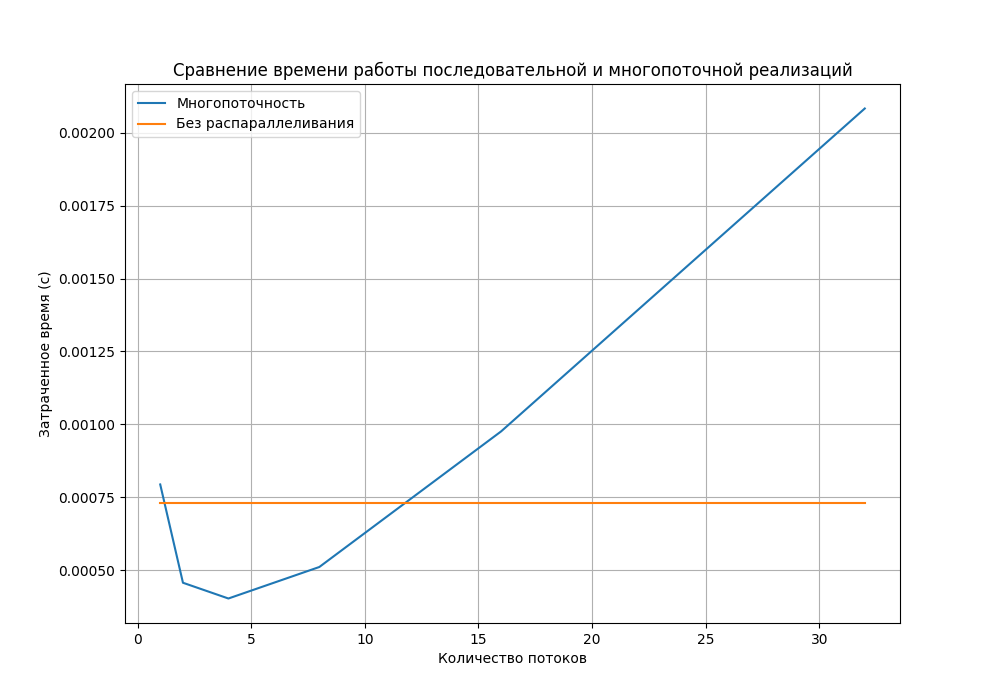
\includegraphics[scale=0.7]{inc/lab4_1v2.png}}
	
	\caption{Сравнение времени работы последовательной и многопоточной реализаций алгоритмов построения спектра отрезков по Брезенехему}
	
	\label{fig:fig1}
	
\end{figure}

\FloatBarrier

На рисунке \ref{fig:fig2} представлено сравнение времени работы реализаций без многопоточности и с 4 потоками алгоритмов построения спектра отрезков по Брезенехему на разных длинах отрезков в спектре.

\FloatBarrier

\begin{figure}[h!]
	
	\centering{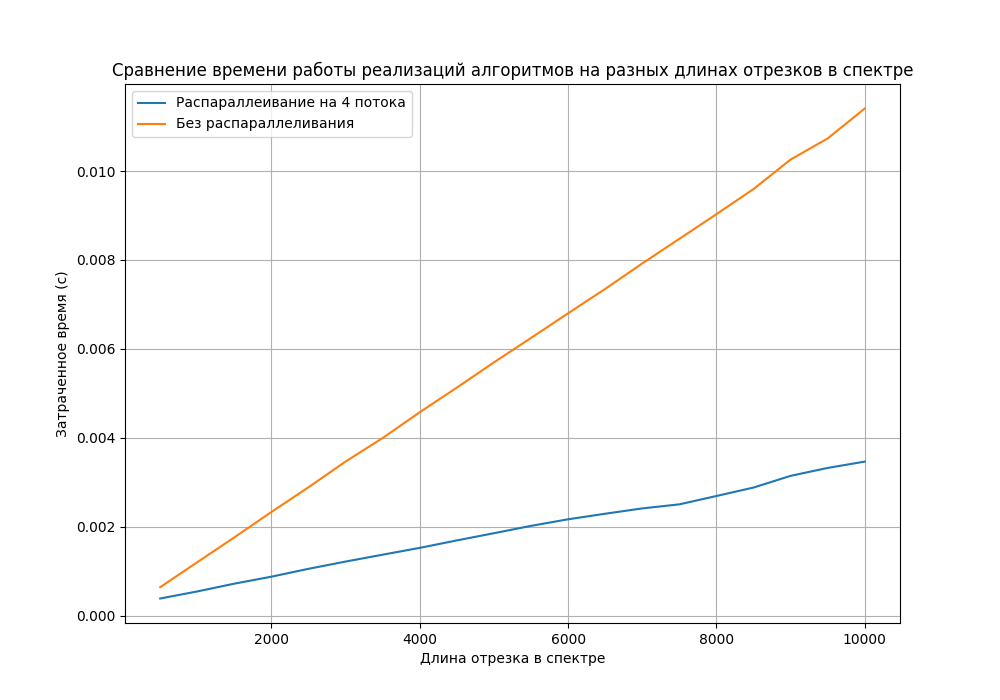
\includegraphics[scale=0.7]{inc/lab4_2.png}}
	
	\caption{Сравнение времени работы реализаций алгоритмов построения спектра отрезков по Брезенехему на разных длинах отрезков в спектре}
	
	\label{fig:fig2}
	
\end{figure}

\clearpage
\FloatBarrier

\section*{Вывод}
В результате эксперимента было получено, что при использовании 4 потоков, многопоточная реализация алгоритма построения спектра отрезков по Брезенехему лучше реализации без многопоточности почти в 2 раза на длине отрезка в спектре, равной 500. Данное количество потоков обусловлено тем, что на ноутбуке, на котором проводились замеры времени, имеется всего 4 логических ядра. Таким образом, рекомендуется применять 4 потока, многопоточная реализация с 4 потоками алгоритма построения спектра отрезков достигает наибольшей эффективности по времени.

Последовательная реализация алгоритма построения спектра отрезков по Брезенхему чуть эффективнее по времени, чем многопоточная реализация с 1 рабочим потоком из-за дополнительных затрат по времени на создание рабочего потока и диспетчеризацию.

Также при проведении эксперимента было выявлено, что при увеличении длины отрезка в спектре, преимущество многопоточной реализации (с 4 потоками) над последовательной растет. Так, при длине отрезка, равной 1000 многопоточная реализация с 4 потоками эффективней по времени реализации без многопоточности в 2.2 раза, а на длине отрезка, равной 10000 --- в 3.3 раза. Следовательно, чем больше длина отрезка в спектре, тем выгоднее использовать многопоточную реализацию.

Важно отметить, что при реализации алгоритма построения спектра отрезков пришлось воспользоваться мьютексом, так как при многопоточной реализации может возникнуть ситуация, когда несколько потоков в один момент времени пытаются закрасить разные пиксели. Таким образом, происходит неопределенное поведение --- часть пискселей закрашивается, а часть --- пропадает. Поэтому была реализована блокировка части кода, которая отвечает за помещение пикселя на канвас с помощью мьютекса. Все вычисления выполняются параллельно, но потокам придется встать в очередь, чтобы закрасить пиксель на экране.